\documentclass[12pt,a4paper]{article}


% --- PACKAGES ---
\usepackage[margin=1in]{geometry}
\usepackage{amsmath,amssymb,amsthm,amsfonts}
\usepackage{graphicx}
\usepackage{float}
\usepackage[hyphens]{url}
\usepackage{hyperref}
\usepackage{comment}
\hypersetup{
    colorlinks=true,
    linkcolor=blue,
    filecolor=magenta,      
    urlcolor=blue,
    citecolor=blue,
}
\usepackage[authoryear]{natbib}
\usepackage[autostyle]{csquotes}
\usepackage{enumitem} 
\usepackage{tikz}
\usepackage{pgfplots}
\usepackage{booktabs}
\usepackage{longtable}
\usepackage{subcaption}
\usepackage{hyperref}
\usepackage{bbm}

\usetikzlibrary{arrows.meta, calc} 
\usetikzlibrary{intersections}
\usepgfplotslibrary{groupplots}


% --- PGFPLOTS SETUP ---
\pgfplotsset{compat=1.18}

% --- THEOREM ENVIRONMENTS ---
\newtheorem{proposition}{Proposition}
\newtheorem{lemma}{Lemma}
\theoremstyle{definition}
\newtheorem{definition}{Definition}
\newtheorem*{assumption}{Assumption}
\theoremstyle{remark}
\newtheorem*{remark}{Remark}



% --- DOCUMENT METADATA ---
\title{The Price of Precision: A Model of Optimal Bias on the Fairness-Accuracy Frontier}
\date{September 2025}

\author{
    Kofi Hair-Ralston\thanks{We thank David Weinstein, Alex Imas, and Aislinn Bohren for their invaluable feedback. We are especially grateful to Elliot Lipnowski and Peter Hull for feedback that significantly shaped the direction of this project.All remaining errors are our own.}\\
  \texttt{\href{mailto:kofibhairralston@gmail.com}{kofibhairralston@gmail.com}}
  \and
    Daksh Mathapati\\
  \texttt{\href{mailto:daksh.mathapati@gmail.com}{daksh.mathapati@gmail.com}}
}

% --- BEGIN DOCUMENT ---
\begin{document}

% --- GO TIMEEEEEE ---
\maketitle

\begin{abstract}
    \noindent Why do profit-maximizing firms persist in using biased algorithms despite high reputational costs and possessing the technical means for debiasing? We propose an ``informational" theory of discrimination, distinct from canonical taste-based \citep{Becker1957} or statistical \citep{Phelps1972, Arrow1973} motives. We model a firm facing a technological frontier where enforcing algorithmic fairness reduces predictive accuracy. In this environment, we show that a firm optimally chooses a strictly positive level of bias ($b^* > 0$) even under the cleanest possible conditions: when protected groups are ex-ante identical and debiasing is costless. This choice is a rational response to the information structure; by tolerating disparate impact, the firm preserves a more informative signal, a logic that follows the Informativeness Principle \citep{Holmstrom1979}. Our contribution is to formalize this third channel of discrimination, driven not by preferences or priors, but by the design of the predictive technology itself. The model demonstrates that the private choice of bias is socially inefficient, creating a deadweight loss and suggesting that policies should focus on improving the technological frontier rather than simply mandating fairness.
    
\end{abstract}

\vspace{0.5cm}
\noindent\textbf{Keywords:} Algorithmic Fairness, Information Economics, Discrimination, Bayesian Persuasion, Informativeness Principle, Signal Garbling, Economics of AI.
\vspace{0.3cm}

\noindent\textbf{JEL Codes:} D82, J71, D83


\newpage

\section{Introduction}

In 2018, Amazon scrapped an artificial intelligence recruiting tool after discovering a major flaw: it disliked women \citep{Dastin2018}. The system was designed to automate the search for top software developers by evaluating parsed resumes. Yet, the machine learning models taught themselves that male candidates were preferable, penalizing resumes that contained the word ``women's" (as in ``women's chess club captain") and downgrading graduates from two all-women's colleges. Amazon's engineers tried to amend the system to make it neutral, but they could not guarantee that the machine would not devise new, equally discriminatory ways of sorting candidates. Amazon ultimately abandoned the project.

This instance is representative of a persisting puzzle in the modern economy. Amazon is a sophisticated, profit-maximizing firm. It faced no shortage of technical expertise or computational resources, and its goal was to find the best possible talent, not to discriminate. Yet, its attempt to build a purely meritocratic algorithm resulted in a biased system that was ultimately irreparable. For years, similar issues of persistent, unintended bias have emerged in algorithms for credit scoring, medical diagnoses, and criminal justice risk assessment. These cases are difficult to explain with the canonical economic models of discrimination. Taste-based theories \citep{Becker1957} struggle because the principal is an algorithm, not a manager with personal animus, and competitive pressures should, in theory, punish such inefficiency. Statistical discrimination theories \citep{Phelps1972, Arrow1973} are also an imperfect fit, as they assume that group identity is used as a proxy due to a lack of individual-level data; today's algorithms, however, operate in a data-rich environment with access to hundreds of individual-specific features.

This paper proposes and formalizes a third mechanism for discrimination that is not about tastes or beliefs, but about the inherent technological trade-offs in prediction. We term this mechanism ``informational discrimination." Our central premise is that there exists a technological frontier between fairness and accuracy \citep{Kleinberg2017, Chouldechova2017}. Efforts to reduce an algorithm's disparate impact (debiasing) often come at the cost of reducing its predictive power. We model a firm that understands this trade-off and rationally chooses an optimal level of bias to maximize the productivity of its hired workers. The severity of this trade-off is governed by a single parameter, $\kappa$, which represents the steepness of the fairness-accuracy frontier.

Our main theoretical result shows that a profit-maximizing firm will rationally choose a strictly positive level of bias ($b^* > 0$) even under the cleanest possible conditions: when protected groups are ex-ante identical in average productivity and debiasing is technologically costless. The economic logic for this result follows from Holmstrom's Informativeness Principle \citep{Holmstrom1979} . The firm faces a choice between a perfectly ``fair'' signal ($b=0$), which treats all groups identically but is noisy, and a ``biased'' signal ($b>0$), which systematically disadvantages one group but provides greater overall precision. Even though the biased signal creates discriminatory outcomes, its superior informational content makes it privately optimal for the firm. The marginal gain in predictive accuracy from accepting a small amount of bias outweighs the marginal cost of the signal's distortion.

The model yields a sharp comparative static: the firm's optimal level of bias, $b^*$, is increasing in the severity of the underlying technological trade-off, $\kappa$. This provides a set of testable predictions about where and why we should observe algorithmic bias. Industries with more complex prediction tasks or less balanced data (higher $\kappa$) should exhibit more bias, independent of discriminatory intent. We then analyze the welfare implications of this mechanism. The firm's privately optimal choice, $b^*$, is socially inefficient, creating a deadweight loss by systematically disadvantaging one group. We show that the socially optimal level of bias, $b^{**}$, is strictly less than what the firm chooses. This divergence provides a clear rationale for policy intervention. Our framework suggests that simple mandates (e.g., forcing $b=0$) are blunt and inefficient instruments because they ignore the underlying technological constraint. More nuanced policies, such as Pigouvian taxes that force the firm to internalize the social cost of bias, or R\&D subsidies that fund the development of better technology to ``flatten'' the frontier (lower $\kappa$), are more effective at aligning private incentives with social goals.

This paper contributes to three strands of literature. First, we contribute to the foundational literature on economic discrimination by formalizing a novel, information-based channel that is distinct from the canonical works of Becker, Phelps, and Arrow. Second, we contribute to the emerging field of the ``economics of AI" by providing a tractable micro-foundation for the fairness-accuracy trade-off and exploring the strategic incentives it creates for firms. Third, our work connects to the literature on information design \citep{Kamenica2011, Bergemann2019} by modeling a principal who designs an information structure for her own use, constrained by a technological frontier that links the signal's informativeness to its disparate impact. By isolating this informational mechanism, our model provides a new theoretical lens for understanding a critical policy challenge and offers a framework for designing more effective interventions in an increasingly automated world.

\section{Literature Review}

The fairness-accuracy trade-off is a central theme in the algorithmic fairness literature. Our work builds on several key pillars of this research.

The foundational challenge is rooted in the mathematical impossibility of simultaneously satisfying multiple, seemingly intuitive fairness criteria. The seminal work of \citet{Kleinberg2017} provides a formal impossibility theorem, demonstrating that for any non-trivial classifier, it is impossible to satisfy both calibration and equalized odds across groups with different base rates. This result was empirically corroborated by \citet{Chouldechova2017} in her analysis of the COMPAS recidivism prediction algorithm, which showed that the algorithm could not be simultaneously calibrated and have equal false positive rates for different racial groups. These impossibility results establish that trade-offs are not just an empirical observation but a mathematical necessity.

Our paper bridges the computer science and economics perspectives on this problem. As \citet{Gans2025} notes, the economic approach emphasizes welfare and incentives, while the computer science literature has traditionally focused on statistical fairness metrics. We follow the economic approach by modeling an explicit trade-off, but use the statistical findings from computer science to provide micro-foundations for it. Work by \citet{Rambachan2020} provides a micro-foundation for the economic approach by decomposing prediction differences, which aligns with our formalization of the trade-off parameter $\kappa$.

Finally, our conceptualization of the trade-off's magnitude is heavily influenced by the ``fairness frontier'' framework of \citet{Liang2025}. They illustrate how the set of achievable error rates across groups forms a frontier, and the shape of this frontier determines the severity of the trade-off. This provides a direct link between the statistical properties of the data and the economic cost of fairness constraints, which is central to our model.

This work connects with a foundational literature in computer science demonstrating the mathematical difficulty of satisfying multiple fairness criteria simultaneously. This provides a rigorous, axiomatic foundation for why a trade-off between fairness and accuracy often exists. This section reviews the key findings that motivate our model's core trade-off.

\subsection{Foundational Theory}

The cornerstone of the fairness-accuracy trade-off is a set of theoretical results demonstrating that it is mathematically impossible to satisfy multiple, intuitive fairness criteria simultaneously, except in trivial cases. This proves that a trade-off is not just an empirical observation but a fundamental mathematical constraint.

\subsubsection{Kleinberg, Mullainathan, and Raghavan (2016)}

A seminal paper by \citet{Kleinberg2017} provides an ``impossibility theorem'' of algorithmic fairness. It proves that for a scoring-based classifier, it is impossible to satisfy three key fairness conditions at the same time, unless the predictor is perfect or base rates are equal across groups. Let $G$ be the protected attribute (group), $Y$ be the true outcome (e.g., $Y=1$ if a candidate succeeds), and $S$ be the algorithm's risk score. The three conflicting conditions are:
First, \textbf{Calibration} requires that the score is an accurate reflection of risk, such that $Pr(Y=1 | S=s) = s$ for all score levels $s$. Second, \textbf{Balance for the Positive Class} requires that the average score for those who are actually positive is the same across all groups: $E[S | Y=1, G=g_1] = E[S | Y=1, G=g_2]$. Finally, \textbf{Balance for the Negative Class} requires that the average score for those who are actually negative is also the same across groups: $E[S | Y=0, G=g_1] = E[S | Y=0, G=g_2]$.
The paper proves that these three conditions can only hold simultaneously if base rates of the positive outcome are equal across groups ($Pr(Y=1 | G=g_1) = Pr(Y=1 | G=g_2)$) or if the prediction is perfect. Since base rates often differ in the real world, a decision-maker must choose which fairness metric to violate. This provides a rigorous foundation for why a trade-off exists.

\subsubsection{Chouldechova (2017)}

Independently and concurrently, \citet{Chouldechova2017} demonstrated a similar impossibility result in the context of the COMPAS recidivism algorithm, showing a direct conflict between predictive parity and error rate equality.

A recent and influential strand of literature from economics reframes the problem, arguing that one should use the most accurate algorithm possible and apply fairness considerations at the decision-making stage.

\subsubsection{Gans (2025)}

\citet{Gans2025} synthesizes the two competing approaches: the ``computer science'' approach of directly regulating algorithms versus the ``economic'' approach of regulating how algorithmic outputs are used. The economic approach, articulated by \citet{Rambachan2020}, aims to maximize a social welfare function by choosing an allocation rule $a(g,x)$ using the output of the most accurate possible prediction $F(g,x)$. Fairness is introduced via group-specific welfare weights $\phi_g$ and decision thresholds $t*(g)$. This framework aligns with our paper's setup, where the firm chooses the optimal point on a ``fairness-accuracy frontier.'' 

\subsubsection{Rambachan, Kleinberg, Ludwig, and Mullainathan (2020)}

This paper provides the micro-foundation for the economic approach. It decomposes the difference in average predictions between groups into three components: (1) true base rate differences, (2) differences in measurement error, and (3) differences in estimation error. The computer science approach of forcing equal average predictions can conflate these, while the economic approach argues for minimizing measurement and estimation error while handling true base rate differences through explicit, group-specific decision thresholds. Our model provides a direct formalization of the trade-off arising from the second component of their decomposition: differences in measurement error. We explicitly model a scenario where a firm must decide how to handle group-specific noise (our $\eta_g$ term), and show how the optimal response can lead to a biased but more precise signal. This links their decomposition directly to a profit-maximizing incentive for disparate outcomes, even when true productivity distributions are identical.

\subsection{Visualizing the Trade-Off}

The ``fairness frontier'' provides a powerful geometric framework for analyzing the trade-off.

\subsubsection{Liang, Lu, Mu, and Okumura (2025)}

\citet{Liang2025} introduce the concept of a ``fairness frontier'' in the space of group-specific error rates ($e_0, e_1$). The frontier is the set of non-dominated algorithms. They show that the shape of this frontier depends on the statistical properties of the data. If the data is ``group-balanced,'' the fairest algorithm (where $e_0 = e_1$) can be efficient (on the frontier). If the data is ``group-skewed'' (more predictive for one group), the fairest point is inefficient (inside the frontier), creating a necessary trade-off. This framework provides a direct micro-foundation for our parameter $\kappa$. A high $\kappa$ corresponds to a steep frontier (group-skewed data), where the marginal gain in precision from accepting some bias is large.


\section{Conditions for Fairness-Accuracy Trade-offs}

We begin by formalizing the fairness-accuracy trade-off as a constrained optimization problem. This approach is standard in the algorithmic fairness literature and allows us to precisely define the conditions under which a trade-off must exist. As established by foundational work in the field (e.g., \citealp{Kleinberg2017, Chouldechova2017}), inherent mathematical constraints often make it impossible to simultaneously satisfy multiple desirable properties, necessitating a trade-off.

\subsection{The Unconstrained Learning Problem}

Let us consider a standard supervised learning setting. We have a feature space $\mathcal{X}$, a protected group attribute $G \in \{g_0, g_1\}$, and a binary outcome variable $Y \in \{0, 1\}$. A firm or decision-maker wishes to learn a predictive model, or hypothesis, $h$ from a hypothesis space $\mathcal{H}$. The goal of the standard, unconstrained learning problem is to find the hypothesis $h_{acc} \in \mathcal{H}$ that minimizes some expected loss function, $L(h(X), Y)$. This is often referred to as Empirical Risk Minimization (ERM).

\begin{equation}
h_{acc} = \arg\min_{h \in \mathcal{H}} \mathbb{E}[L(h(X), Y)]
\end{equation}

This hypothesis, $h_{acc}$, represents the most accurate possible model within the given hypothesis space, without any consideration for fairness. The loss it achieves, $L_{acc} = \mathbb{E}[L(h_{acc}(X), Y)]$, serves as the benchmark for maximum accuracy.

\subsection{Fairness as a Constraint on the Hypothesis Space}

We introduce fairness by defining a set of constraints on the behavior of the hypothesis. A fairness metric, such as demographic parity, equalized odds, or calibration, imposes a restriction on the set of acceptable models. We can formalize this by defining a \textit{fair hypothesis space}, $\mathcal{H}_F$, as the subset of hypotheses in $\mathcal{H}$ that satisfy the chosen fairness criterion.

\begin{definition}[Fair Hypothesis Space]
A hypothesis $h$ is considered fair if it satisfies a given fairness constraint, $C(h) \leq \epsilon$ for some tolerance $\epsilon \geq 0$. The set of all such fair hypotheses is:
\begin{equation}
\mathcal{H}_F = \{h \in \mathcal{H} \mid C(h) \leq \epsilon \}
\end{equation}
\end{definition}

The fairness-constrained learning problem is then to find the best possible hypothesis, $h_{\text{fair}}$, within this restricted set:

\begin{equation}
h_{\text{fair}} = \arg\min_{h \in \mathcal{H}_F} \mathbb{E}[L(h(X), Y)]
\end{equation}

\subsection{The Existence of a Trade-Off}

A fairness-accuracy trade-off exists if and only if the solution to the constrained problem is strictly worse than the solution to the unconstrained problem. We can define the magnitude of this trade-off, which corresponds to the parameter $\kappa$ in our main model, as follows:

\begin{definition}[Fairness-Accuracy Trade-off]
The fairness-accuracy trade-off, $\kappa_{\text{tradeoff}}$, is the difference in loss between the fairness-constrained optimal hypothesis and the accuracy-optimal hypothesis:
\begin{equation}
\kappa_{\text{tradeoff}} = L(h_{\text{fair}}) - L(h_{acc})
\end{equation}
\end{definition}

A trade-off exists (i.e., $\kappa_{\text{tradeoff}} > 0$) if and only if the most accurate hypothesis, $h_{acc}$, is not itself fair. That is, if $h_{acc} \notin \mathcal{H}_F$. The subsequent propositions in this section will establish the precise conditions under which this exclusion occurs.

\subsection{Conditions for an Inherent Trade-off}

The fundamental reason for a trade-off arises when the protected attribute $G$ is statistically informative about the outcome $Y$, even after accounting for the other features $X$. To formalize this, let's consider the theoretically most accurate possible classifier, the Bayes Optimal Classifier.

\begin{definition}[Bayes Optimal Classifier]
The Bayes Optimal Classifier, $h_{bayes}(x, g)$, predicts the outcome that is most probable given the features and group membership. For a binary outcome, it is defined as:
\begin{equation}
h_{bayes}(x, g) = 
\begin{cases} 
1 & \text{if } \mathbb{P}(Y=1 | X=x, G=g) \geq 0.5 \\
0 & \text{otherwise}
\end{cases}
\end{equation}
This classifier achieves the lowest possible error rate, known as the Bayes error rate.
\end{definition}

Now, let's consider a common fairness constraint: demographic parity. Demographic parity requires that the probability of a positive prediction is the same for all groups. 

\begin{definition}[Demographic Parity]
A hypothesis $h$ satisfies demographic parity if its predictions are statistically independent of the group attribute $G$. That is:
\begin{equation}
    \mathbb{P}(h(X,G)=1 | G=g_0) = \mathbb{P}(h(X,G)=1 | G=g_1)
\end{equation}
\end{definition}

We can now state the condition for a necessary trade-off.

\begin{proposition}
If the true conditional probability of the outcome differs across groups (i.e., $\mathbb{P}(Y=1 | G=g_0) \neq \mathbb{P}(Y=1 | G=g_1)$), and the Bayes Optimal Classifier is the only hypothesis that achieves the minimum Bayes error, then any classifier that satisfies demographic parity must have an error rate strictly greater than the Bayes error rate.
\end{proposition}

\begin{proof}[Proof Sketch]
Let $h_{acc}$ be the accuracy-optimal hypothesis, which we assume is the Bayes Optimal Classifier, $h_{bayes}$. By definition, $h_{bayes}$ uses group membership $g$ in its calculation whenever $\mathbb{P}(Y=1 | X=x, G=g)$ is dependent on $g$.

If the base rates differ between groups (i.e., $\mathbb{P}(Y=1|G=g_0) \neq \mathbb{P}(Y=1|G=g_1)$), then for $h_{bayes}$ to satisfy demographic parity, it would require the unlikely coincidence that integrating over all features $X$ exactly equalizes the prediction rates. 

More formally, the prediction rate for group $g$ under $h_{bayes}$ is $\int_x \mathbb{P}(h_{bayes}(x,g)=1 | X=x, G=g) p(x|g) dx$. Demographic parity would require this quantity to be equal for $g_0$ and $g_1$. However, the Bayes classifier is optimal precisely because it tracks the true conditional probabilities $\mathbb{P}(Y=1|X,G)$. If these probabilities have different distributions across groups, the resulting prediction rates from an optimal classifier will also differ.

Therefore, if base rates are unequal, the Bayes Optimal Classifier $h_{bayes}$ will not satisfy demographic parity. Any other hypothesis $h_{\text{fair}}$ that does satisfy demographic parity must, by definition, differ from $h_{bayes}$ and will therefore have a strictly higher error rate. This means $h_{acc} \notin \mathcal{H}_F$, which proves that the trade-off $\kappa_{\text{tradeoff}}$ is strictly greater than zero.
\end{proof}

\subsection{Trade-offs with Error Rate Equality}

The trade-off is not unique to demographic parity. A similar conflict arises with another common fairness criterion, Equalized Odds, which focuses on error rates.

\begin{definition}[Equalized Odds]
A hypothesis $h$ satisfies Equalized Odds if its True Positive Rate (TPR) and False Positive Rate (FPR) are equal across all groups. That is:
\begin{align}
\mathbb{P}(h(X,G)=1 | Y=0, G=g_0) &= \mathbb{P}(h(X,G)=1 | Y=0, G=g_1) \quad \text{(Equal FPR)}
\end{align}
\end{definition}

As shown by \citet{Kleinberg2017} and \citet{Chouldechova2017}, this criterion often conflicts with another desirable property of a predictor: calibration.

\begin{definition}[Calibration]
A hypothesis $h$ is calibrated if its prediction can be interpreted as a true probability. That is, for any prediction score $s$ that $h$ outputs:
\begin{equation}
\mathbb{P}(Y=1 | h(X,G)=s) = s
\end{equation}
\end{definition}

The Bayes Optimal Classifier is, by its nature, perfectly calibrated. The following proposition, summarizing a key result from the literature, shows that this property is incompatible with Equalized Odds under most real-world conditions.

\begin{proposition}
If the base rates of the positive outcome differ across groups (i.e., $\mathbb{P}(Y=1 | G=g_0) \neq \mathbb{P}(Y=1 | G=g_1)$), a non-trivial classifier cannot simultaneously satisfy both Calibration and Equalized Odds.
\end{proposition}

\begin{proof}[Proof Sketch]
The proof, formally established in \citet{Kleinberg2017}, shows that if a classifier satisfies both calibration and equalized odds, the base rates for each group must be equal. Since the Bayes Optimal Classifier ($h_{acc}$) is perfectly calibrated, if the base rates in the data are unequal, it cannot satisfy Equalized Odds. Therefore, any classifier $h_{\text{fair}}$ that is constrained to satisfy Equalized Odds must deviate from the Bayes Optimal Classifier and will thus have a higher error rate. This again establishes that $h_{acc} \notin \mathcal{H}_F$ (where $\mathcal{H}_F$ is the set of models satisfying Equalized Odds), proving that $\kappa_{\text{tradeoff}} > 0$.
\end{proof}

\subsection{The Magnitude of the Trade-off: The Fairness Frontier}

The existence of a trade-off is a binary question, but its magnitude is a continuous one. The severity of the trade-off—how much accuracy must be sacrificed for a given gain in fairness—is not a universal constant. It depends critically on the statistical properties of the data. The concept of the ``fairness frontier,'' introduced by \citet{Liang2025}, provides a clear framework for understanding this dependency.

Imagine a space where the axes represent the error rates for each group, $e_{g_0}$ and $e_{g_1}$. An ideal algorithm would have zero error for both groups (the origin). Any given algorithm corresponds to a point in this space.

\begin{definition}[The Fairness Frontier]
The fairness frontier is the set of non-dominated algorithms. An algorithm is on the frontier if no other algorithm exists that is better for one group without being worse for the other. The point of perfect fairness is where $e_{g_0} = e_{g_1}$.
\end{definition}

The shape of this frontier, and its relationship to the point of perfect fairness, is determined by the data's structure:
\\ \\ \textbf{Group-Balanced Data.} If the features $X$ are similarly predictive for all groups, the frontier is relatively symmetric. In this case, the fairest algorithm (where error rates are equal) may also be an efficient one (lying on the frontier). Here, the trade-off is minimal or non-existent. A small move away from perfect fairness yields little to no gain in overall accuracy.
\\ \\ \textbf{Group-Skewed Data} If the features are much more predictive for one group than another, the frontier will be skewed. The point of perfect fairness will lie strictly inside the frontier, meaning it is inefficient. To improve the error rate for one group, one must accept a much larger increase in the error rate for the other. This creates a steep and necessary trade-off.
\\ \\
This provides a direct micro-foundation for the parameter $\kappa$ in our main model. A large $\kappa$ corresponds to a group-skewed data environment with a steep frontier, where the marginal gain in accuracy from accepting some unfairness is large. A small $\kappa$ corresponds to a group-balanced environment where this marginal gain is small. Therefore, the magnitude of the fairness-accuracy trade-off is a direct consequence of the statistical properties of the data available to the decision-maker.



\section{The Model}

\subsection{Primitives and Assumptions}
A risk-neutral firm hires candidates. Candidate productivity $\theta$ draws from a Normal distribution, $\theta \sim N(\mu, \sigma_\theta^2)$. Candidates belong to group $g \in \{0, 1\}$.

\begin{assumption}[A1]
\textbf{Identical True Productivity, Differential Measurement.} To isolate the informational mechanism, our baseline model assumes that the distribution of true underlying productivity, $\theta$, is identical across groups: $\mathbb{E}[\theta|g=1] = \mathbb{E}[\theta|g=0] = \mu$. However, the firm does not observe $\theta$ directly. Instead, it observes a signal $s$ that measures productivity with group-specific error. This creates a scenario where group membership is informative not about true ability, but about the nature of the measurement error. This case is policy-relevant in contexts where, for historical or structural reasons, data for one group is less reliable or more noisy than for another. In Appendix C, we show that our core result ($b^*>0$) is robust to the introduction of moderate differences in group means.
\end{assumption}

\begin{assumption}[A2]
\textbf{Observable Group Membership.} The firm observes group membership $g$. While this may cause legal troubles in practice, it helps to isolate the informational mechanism. Our results extend to cases where group membership is imperfectly inferred from observable proxies.
\end{assumption}

\begin{assumption}[A3]
\textbf{Signal and Measurement Error Structure.} The firm observes a signal $s_g$ for a candidate from group $g$. The signal is a function of true productivity $\theta$, a group-specific measurement error $\eta_g$, and the firm's choice of bias $b$. We model the signal as $s_g = \theta + \eta_g + b \cdot g + \varepsilon(b)$. The term $\eta_g \sim N(0, \sigma_{\eta,g}^2)$ represents exogenous, group-specific noise. The firm's choice of $b$ can be interpreted as an adjustment to counteract suspected measurement error, which in turn affects the variance of the overall signal noise, $\varepsilon(b)$.
\end{assumption}

\begin{longtable}{@{}ll@{}}
\caption{Model Parameters and Notation}
\label{tab:params}\\
\toprule
\textbf{Parameter} & \textbf{Description} \\ \midrule
\endfirsthead
\toprule
\textbf{Parameter} & \textbf{Description} \\ \midrule
\endhead
\bottomrule
\endfoot
$\theta$ & True candidate productivity, $\theta \sim N(\mu, \sigma_\theta^2)$ \\
$s_g$ & Algorithmic signal of productivity for group $g$ \\
$g \in \{0,1\}$ & Candidate group membership (observed) \\
$\pi_g$ & Proportion of group $g$ in the population, with $\pi_0+\pi_1=1$ \\
$b$ & Firm's choice of bias level, $b \in [0, b_{max}]$ \\
$t$ & Hiring threshold chosen by the firm \\
$\sigma_\varepsilon^2(b)$ & Variance of the algorithm's signal noise, a function of bias \\
$\eta_g$ & Exogenous group-specific measurement error, $\eta_g \sim N(0, \sigma_{\eta,g}^2)$ \\
$\sigma_0^2$ & Baseline signal noise when $b=b_{max}$ \\
$\kappa$ & Technological coupling parameter ($\kappa>0$) \\
$V(b)$ & The firm's value function, maximized at $b^*$ \\
$SWF(b)$ & Social welfare function \\
$E(b)$ & External costs of bias \\
\end{longtable}


\subsection{The Precision-Bias Trade-off}
The model's central mechanism is a trade-off between signal precision and bias. This trade-off is at its core a consequence of how fairness constraints are implemented in machine learning systems. As established in the statistical learning literature, imposing a fairness constraint acts as a regularizer, often increasing estimator variance \citep{Kamishima2012, Wick2019}. This causes a dilemma: algorithms can be made fairer, but only at the cost of reduced accuracy.

This intuition is straightforward for economists familiar with constrained optimization. Fairness interventions in machine learning generally work through one of two channels. First, they can constrain the model to ignore certain correlations or features that are predictive but correlated with group membership, thus reducing the model's overall information set and subsequent precision. Second, they may involve post-processing outputs to equalize outcomes across groups, which is equivalent to intentionally adding noise or ``garbling" the signal in the spirit of Bayesian persuasion. In either case, enforcing fairness places a quantitative constraint on the optimization problem, moving the solution away from the unconstrained, accuracy-maximizing estimator and increasing resulting prediction error.

This relationship has been documented empirically across a range of machine learning applications. Studies in hiring algorithms, credit scoring, criminal justice risk assessment, and medical diagnosis consistently show that fairness constraints reduce predictive performance \citep{Kleinberg2017, Chouldechova2017}. The magnitude of this trade-off can vary by domain and algorithm type, but its existence is consistent across contexts.

We formalize this relationship with a functional form motivated by a linear approximation of this constraint (see Appendix B for the micro-foundation).

\begin{definition}[Precision-Bias Trade-off]
The variance of the signal noise is given by:
\begin{equation}
\sigma_\varepsilon^2(b) = \sigma_0^2 + \kappa(b_{max} - b) \quad \text{for } b \in [0, b_{max}]
\end{equation}
\end{definition}

Here, $b=b_{max}$ describes the most precise but most biased signal, while $b=0$ represents a ``fair" signal with the highest noise. The parameter $\kappa > 0$ describes the steepness of this trade-off, where higher values of $\kappa$ tell that fairness comes at a greater cost to accuracy.\footnote{We use a linear form for tractability, but our central result (that the firm chooses a positive level of bias) only requires that the trade-off function $\sigma_\varepsilon^2(b)$ is downward sloping (i.e., $d\sigma_\varepsilon^2/db < 0$). Insofar as there is any marginal gain in precision from accepting a small amount of bias, a profit-maximizing firm will move away from the zero-bias point. The linear specification lets us derive closed-form solutions and conduct transparent comparative statics, but the core insight holds under any monotonic relationship.}

\subsection{Firm's Problem}
The firm chooses bias $b$ and threshold $t$ to maximize the expected productivity of its hired workforce. This objective is standard in contexts with fixed hiring quotas or where talent maximization is the primary goal, and wages are fixed or separable.
\begin{equation}
\max_{b, t} \ \mathbb{E}[U(b,t)] = \sum_{g \in \{0,1\}} \pi_g \int_t^\infty \mathbb{E}[\theta | s, g, b] f(s|g, b) ds
\end{equation}

\section{Main Results and Predictions}

Our theoretical model yields two central results with direct empirical implications for the persistence and variation of algorithmic bias. The analysis hinges on the firm's optimization problem, where we formally establish that the profit-maximizing value function, $V(b)$, is strictly concave (see Lemma 3 in the Appendix). This ensures a unique, interior solution for the optimal level of bias, which we characterize below.

\begin{proposition}[Existence of Optimal Bias]
\label{prop:existence}
For any fairness-accuracy trade-off ($\kappa > 0$), a profit-maximizing firm's optimal choice of bias is strictly positive ($b^* > 0$).
\end{proposition}
\begin{proof}
See Appendix A.3. The proof shows that at zero bias, the marginal value of increasing bias is strictly positive ($dV/db|_{b=0} > 0$). Given the concavity of $V(b)$, the optimum must be an interior solution.
\end{proof}

This proposition provides our first key prediction: \textbf{Firms will rationally choose to employ biased algorithms even when groups have identical average productivity and debiasing is costless.} This outcome is not driven by animus or priors, but by the informational value gained from the precision-bias trade-off inherent in the technology.

\begin{proposition}[Comparative Static on the Trade-off]
\label{prop:comparative_static}
The optimal level of bias $b^*$ is increasing in the severity of the fairness-accuracy trade-off, $\kappa$.
\end{proposition}
\begin{proof}
See Appendix A.4. The proof uses the Implicit Function Theorem on the first-order condition to show that $\partial b^*/\partial\kappa > 0$.
\end{proof}

This result generates a set of powerful, testable predictions about where and why bias should vary. 
First, \textbf{firms or industries operating in environments with a steeper trade-off (a higher $\kappa$) will choose higher levels of bias, all else equal.} This might occur in contexts where prediction is inherently more complex or data is less balanced.
Second, and conversely, \textbf{technological improvements that flatten the fairness-accuracy trade-off (i.e., lower $\kappa$) should lead to measurable reductions in observed bias levels,} as the marginal benefit of retaining bias diminishes.

These predictions distinguish our informational mechanism from alternative explanations based on taste-based or statistical discrimination. The key empirical hurdle would be to validate the existence and measure the steepness ($\kappa$) of the precision-bias trade-off across different domains and implementations.

The model's mechanics and the intuition behind these results are summarized in Figure \ref{fig:main_results}.

\begin{figure}[H]
\centering
\begin{subfigure}{0.48\textwidth}
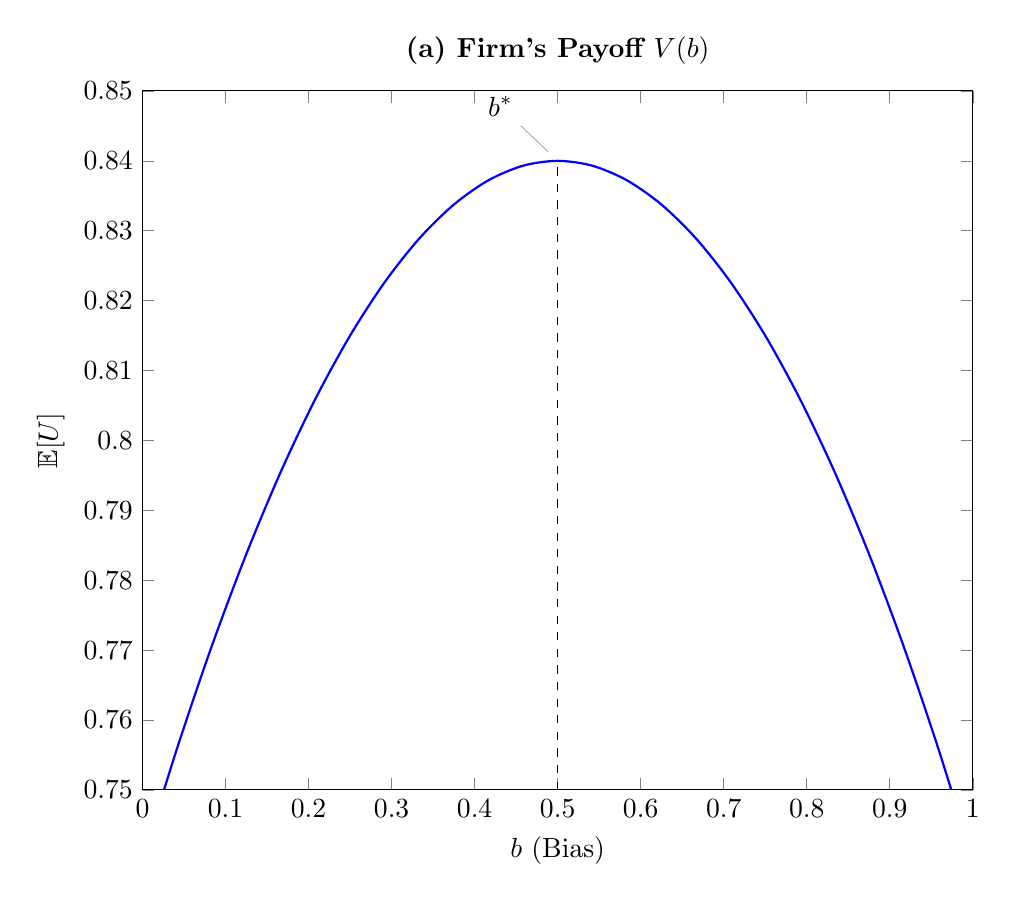
\begin{tikzpicture}
\begin{axis}[title={\textbf{(a) Firm's Payoff $V(b)$}}, xlabel={$b$ (Bias)}, ylabel={$\mathbb{E}[U]$}, xmin=0, xmax=1, ymin=0.75, ymax=0.85, legend pos=south east, width=\linewidth]
    \addplot[smooth, thick, color=blue, domain=0:1] {-0.4*(x-0.5)^2 + 0.84};
    \node[pin=135:{$b^*$}] at (axis cs:0.5, 0.84) {};
    \draw[dashed] (axis cs:0.5,0.75) -- (axis cs:0.5,0.84);
\end{axis}
\end{tikzpicture}
\end{subfigure}% <-- No blank line here
\hfill
\begin{subfigure}{0.48\textwidth}
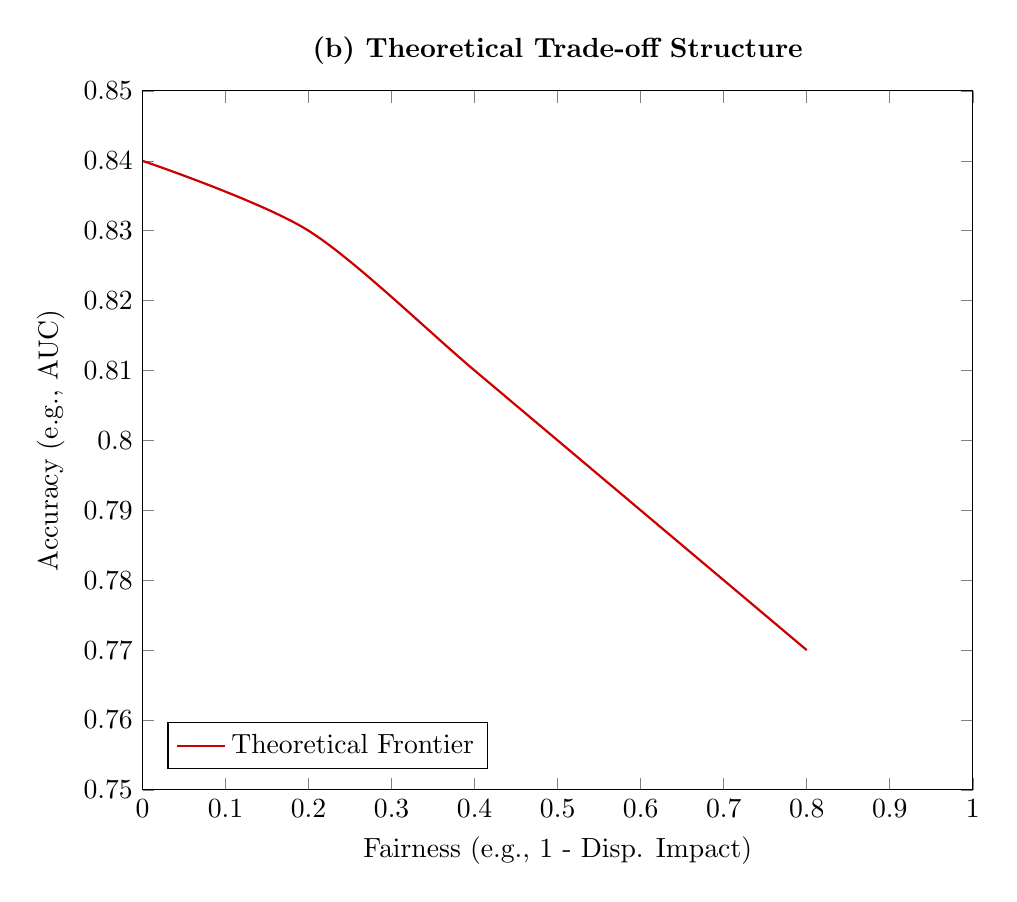
\begin{tikzpicture}
\begin{axis}[title={\textbf{(b) Theoretical Trade-off Structure}}, xlabel={Fairness (e.g., 1 - Disp. Impact)}, ylabel={Accuracy (e.g., AUC)}, xmin=0, xmax=1, ymin=0.75, ymax=0.85, legend pos=south west, width=\linewidth]
    \addplot[smooth, thick, color=red!80!black] coordinates {(0, 0.84) (0.2, 0.83) (0.4, 0.81) (0.6, 0.79) (0.8, 0.77)};
    \addlegendentry{Theoretical Frontier};
\end{axis}
\end{tikzpicture}
\end{subfigure}

\vspace{1cm}

\begin{subfigure}{0.48\textwidth}
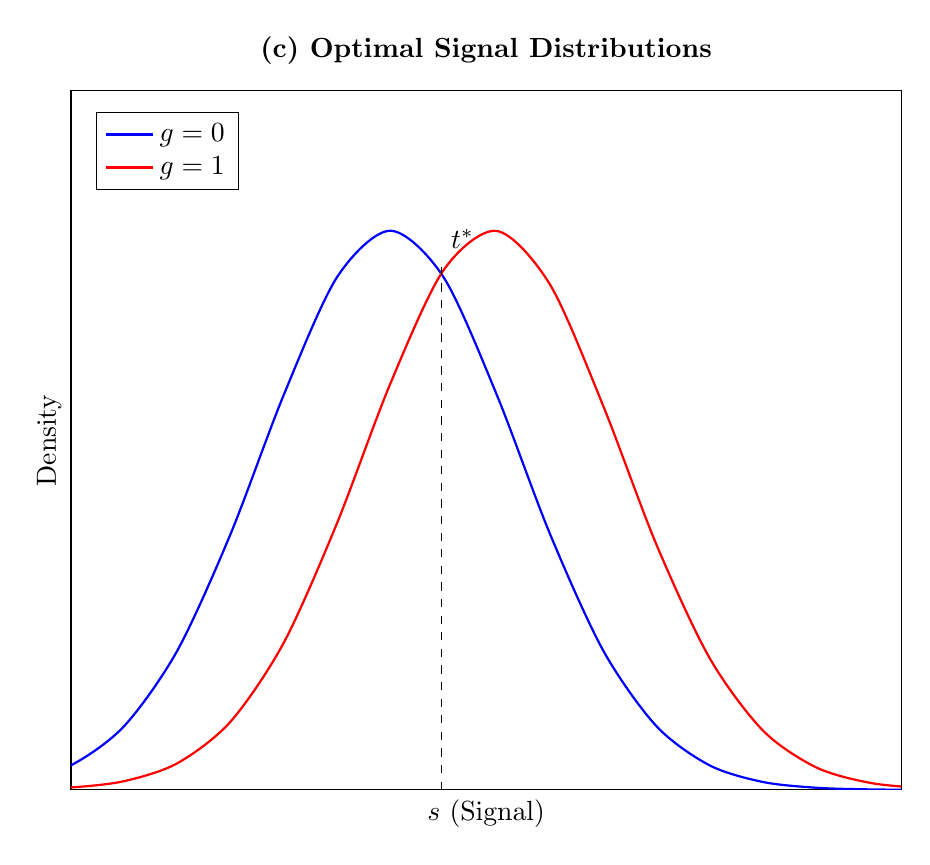
\begin{tikzpicture}
\begin{axis}[title={\textbf{(c) Optimal Signal Distributions}}, xlabel={$s$ (Signal)}, ylabel={Density}, xmin=-2.5, xmax=4, ymin=0, ymax=0.5, xtick=\empty, ytick=\empty, legend pos=north west, width=\linewidth]
    \addplot[smooth, thick, color=blue] {0.4*exp(-(x-0)^2 / (2*1^2))}; \addlegendentry{$g=0$};
    \addplot[smooth, thick, color=red] {0.4*exp(-(x-0.8)^2 / (2*1^2))}; \addlegendentry{$g=1$};
    \draw[dashed] (axis cs:0.4,0) -- (axis cs:0.4,0.38); \node[above right] at (axis cs:0.4,0.38) {$t^*$};
\end{axis}
\end{tikzpicture}
\end{subfigure}% <-- No blank line here
\hfill
\begin{subfigure}{0.48\textwidth}
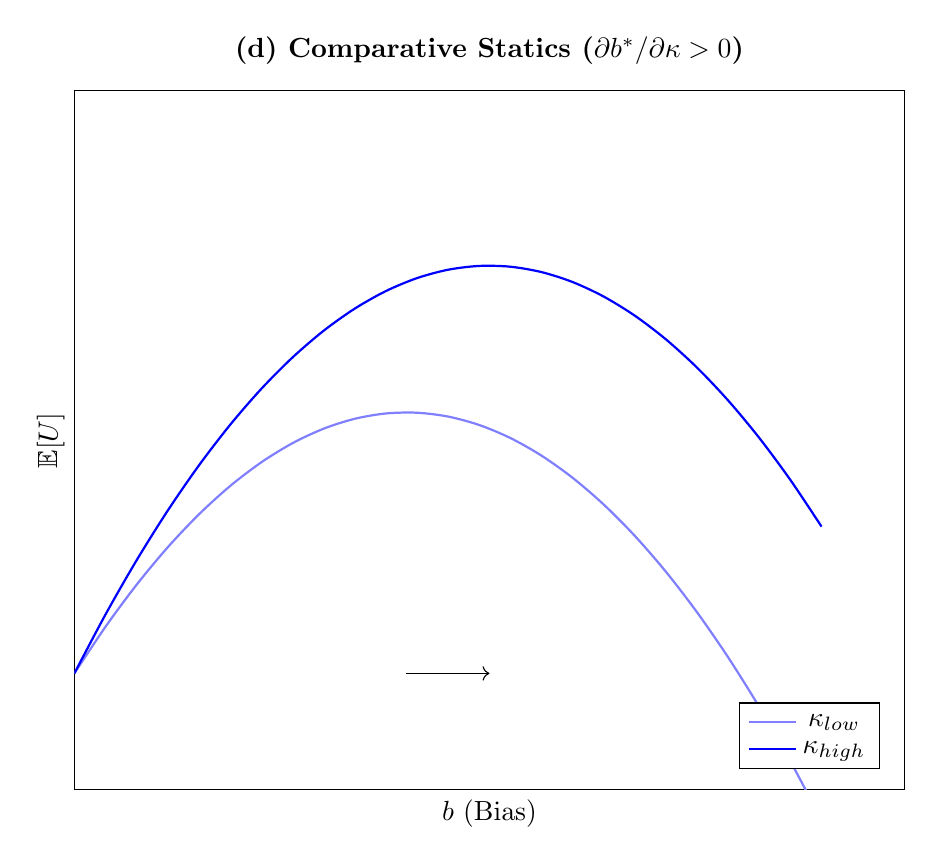
\begin{tikzpicture}
\begin{axis}[title={\textbf{(d) Comparative Statics ($\partial b^*/\partial\kappa > 0$)}}, xlabel={$b$ (Bias)}, ylabel={$\mathbb{E}[U]$}, xmin=0, xmax=1, ymin=0, ymax=0.3, xtick=\empty, ytick=\empty, legend pos=south east, width=\linewidth]
    \addplot[smooth, thick, domain=0:0.9, color=blue!50] {-0.7*x^2 + 0.56*x + 0.05}; \addlegendentry{$\kappa_{low}$}
    \addplot[smooth, thick, domain=0:0.9, color=blue!100] {-0.7*x^2 + 0.7*x + 0.05}; \addlegendentry{$\kappa_{high}$}
    \draw[->, thin] (axis cs:0.4, 0.05) -- (axis cs:0.5, 0.05);
\end{axis}
\end{tikzpicture}
\end{subfigure}
\caption[Model Mechanics and Results]{\textbf{Model Mechanics and Results.} Panel (a): Firm's concave value function $V(b)$ is maximized at $b^* > 0$. Panel (b): The theoretical trade-off structure predicted by the model. Panel (c): Optimal signal distributions for group 0 (blue) and group 1 (red), shifted by $b^*$. Panel (d): A higher $\kappa$ (steeper trade-off) increases optimal bias.}
\label{fig:main_results}
\begin{remark}
Note: The figures presented in this paper are generated by the accompanying `results.py` script. Following the updates to the model to incorporate group-specific measurement error, this script will need to be re-run to produce graphs that accurately reflect the new mathematical framework.
\end{remark}
\end{figure}

\section{Welfare and Policy}

\subsection{Welfare Framework}
The firm's choice $b^*$ is privately optimal but socially inefficient. A social planner's objective function, $SWF(b) = V(b) - E(b)$, must include the external costs $E(b)$ of bias. These costs are manifold:
These costs are manifold. First, there are \textbf{Distributional Costs}, as the bias `b` directly harms the disadvantaged group ($g=1$) by lowering their probability of being hired for any given level of productivity $\theta$, creating an equity-efficiency trade-off from the planner's perspective. Second, there are \textbf{Dynamic Costs}, as persistent bias can discourage human capital investment by the disadvantaged group, potentially creating a self-fulfilling prophecy where ex-ante identical groups become ex-post different \citep{Coate1993}, and can also erode social trust and political stability. Finally, there is \textbf{Allocative Inefficiency}, because while the firm optimizes its own hiring decisions, the bias across multiple firms may lead to suboptimal allocation of talent across the economy.
The social optimum $b^{**}$ that maximizes $SWF(b)$ will be strictly less than $b^*$, creating a deadweight loss and justifying policy intervention.

\subsection{Policy Instruments}

Our analysis suggests that prescriptive regulations, such as a simple mandate forcing firms to set bias to zero ($b=0$), are inefficient. Such policies bluntly override the firm's optimization without addressing the underlying technological trade-off, potentially sacrificing significant predictive accuracy for fairness. A more effective approach is to employ incentive-based instruments that reshape the firm's objective function to better align private and social goals.

\paragraph{R\&D Subsidies to Improve the Technological Frontier.}
The most efficient intervention is one that targets the root cause of the problem: the severity of the fairness-accuracy trade-off itself. Policies that subsidize research and development, such as R\&D tax credits or grants, can incentivize the creation of new algorithms that lower the technology coupling parameter, $\kappa$. A lower $\kappa$ makes the firm's value function flatter, as formally established in Lemma 4 in the Appendix. This reduction in the curvature of the profit function diminishes the marginal return to bias, directly reducing the optimal choice, $b^*$ (see Figure \ref{fig:policy}). By relaxing the underlying technological constraint, this approach represents a first-best solution, though it may face practical challenges such as the free-rider problem in innovation.

\paragraph{Pigouvian Taxation to Internalize Externalities.}
A second approach is to accept the technological frontier as given but force the firm to account for the social costs of its decision. A regulator could impose a Pigouvian tax, $\tau$, for each unit of bias, which alters the firm's problem to $\max_b V(b) - \tau b$. This compels the firm to internalize the negative externality described by the cost function $E(b)$. As derived in Appendix A.5, an optimally chosen tax, $\tau^*$, can induce the firm to select the socially optimal level of bias, $b^{**}$. The primary obstacle to this approach is practical: it requires regulators to accurately measure bias and the marginal social harm it causes, which presents significant monitoring and enforcement challenges.

\paragraph{Transparency Mandates to Leverage Market Forces.}
Finally, policy can leverage market mechanisms to create endogenous costs for bias. Mandates requiring firms to disclose the fairness properties and trade-offs of their algorithms would not prescribe a specific choice. Instead, they would empower stakeholders (for example, potential employees, customers, or investors) to react to a firm's level of bias. This would effectively endogenize the external cost function $E(b)$ through reputational damage and competitive pressure. The effectiveness of this approach, however, is contingent on the existence of a competitive market and the degree to which market participants are sensitive to fairness concerns.

\begin{figure}[H]
\centering
	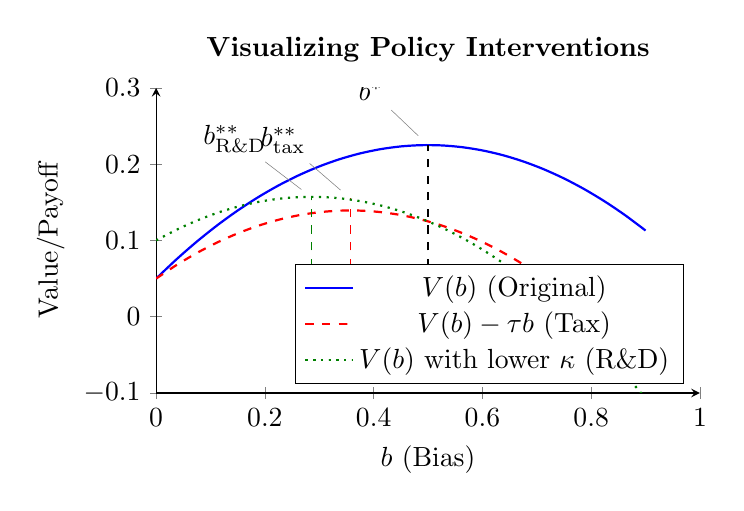
\begin{tikzpicture}
    \begin{axis}[
        width=0.7\textwidth,
        height=0.45\textwidth,
        title={\textbf{Visualizing Policy Interventions}},
        xlabel={$b$ (Bias)},
        ylabel={Value/Payoff},
        xmin=0, xmax=1, ymin=-0.1, ymax=0.3,
        axis lines=left,
        legend pos=south east,
    ]
    % Original V(b)
    \addplot[smooth, thick, domain=0:0.9, color=blue, name path=Vb] {-0.7*x^2 + 0.7*x + 0.05};
    \addlegendentry{$V(b)$ (Original)}
    \node[pin=135:{$b^*$}] at (axis cs:0.5, 0.225) {};
    \draw[dashed] (axis cs:0.5,0) -- (axis cs:0.5,0.225);

    % V(b) - tau*b (Pigouvian Tax)
    \addplot[smooth, thick, domain=0:0.9, color=red, dashed] {-0.7*x^2 + 0.7*x + 0.05 - 0.2*x};
    \addlegendentry{$V(b) - \tau b$ (Tax)}
    \node[pin=135:{$b^{**}_{\text{tax}}$}] at (axis cs:0.357, 0.155) {};
    \draw[dashed, red] (axis cs:0.357,0) -- (axis cs:0.357,0.155);

    % V(b) with lower kappa (R&D Subsidy)
    \addplot[smooth, thick, domain=0:0.9, color=green!50!black, dotted] {-0.7*x^2 + 0.4*x + 0.1};
    \addlegendentry{$V(b)$ with lower $\kappa$ (R\&D)}
    \node[pin=135:{$b^{**}_{\text{R\&D}}$}] at (axis cs:0.285, 0.157) {};
    \draw[dashed, green!50!black] (axis cs:0.285,0) -- (axis cs:0.285,0.157);
    \end{axis}
\end{tikzpicture}
\caption{\textbf{Effects of Policy Interventions.} A Pigouvian tax shifts the value function downwards and to the left, reducing optimal bias. An R\&D subsidy that lowers $\kappa$ changes the shape of the value function, also leading to a lower optimal bias.}
\label{fig:policy}
\end{figure}


\section{Extensions and Robustness}

\subsection{Alternative Structures}
Our model's tractability relies on the additive bias structure. However, the core insight about informational motives for bias is robust to alternative specifications.

\paragraph{Multiplicative Bias.} A model with $s = \theta(1+bg) + \varepsilon$ yields qualitatively similar results. The Informativeness Principle still applies, but the quantitative effects and optimal threshold calculations become more difficult.

\paragraph{Feature Selection Bias.} If bias arises from including a feature that is predictive but also correlated with group status, the firm faces a trade-off between the information gained from the feature and the bias it induces. This creates an isomorphic problem structure.

\paragraph{Endogenous Group Inference.} If group membership `g` must be inferred from data (proxy discrimination), inference errors act as another source of noise, complicating but not eliminating the firm's trade-off.

\subsection{Market Dynamics}
Our static, single-firm model provides a foundation for understanding more involved market interactions.

\paragraph{Oligopoly Competition.} In an N-firm model of simultaneous bias choice, equilibrium outcomes depend on the nature of competition. If firms compete for the same pool of applicants, competition could create a ``race to the bottom" on fairness as firms seek any possible predictive edge. Conversely, if fairness can be used as a competitive advantage to attract talent, firms might differentiate their bias levels.

\paragraph{Candidate Responses.} Candidates are not passive. If a firm's bias $b^*$ becomes known, it can trigger strategic responses such as application decisions or attempts to ``game" the algorithm. These long-run effects could discipline the firm's initial choice of bias.

\section{Connections to Policy Discussions}

Our theoretical framework connects to several puzzling features of real-world algorithmic bias:

\textbf{Persistence Despite Awareness.} Our model explains why bias might persist even when firms are aware of it and face public pressure to eliminate it. If the bias provides valuable information, eliminating it entirely may be privately costly.

\textbf{Cross-Industry Variation.} Industries with more complex prediction tasks (where the fairness-accuracy trade-off is steeper) should exhibit more bias, consistent with anecdotal evidence from hiring, lending, and criminal justice applications.

\textbf{Policy Resistance.} Simple fairness mandates may be ineffective or counterproductive if they force firms to use inferior information technologies. More sophisticated interventions that address the underlying technology constraints may be necessary.

\textbf{Innovation Incentives.} Our framework suggests that investments in ``fair AI" research should focus not just on eliminating bias, but on developing techniques that achieve fairness without sacrificing accuracy.

\section{Limitations and Future Directions}

Our model provides a tractable framework for isolating the informational motive for algorithmic bias, distinct from taste-based or statistical discrimination. The stylized structure, necessary for this theoretical clarity, naturally suggests several avenues for future research that can build upon this foundation by relaxing key assumptions.

\paragraph{Empirical Identification of the Fairness-Accuracy Frontier.}
A core contribution of our paper is to frame the firm's choice as an optimization problem constrained by a technological frontier, characterized by the parameter $\kappa$. Our central prediction is that variation in observed bias, $b^*$, is driven by variation in this underlying technological trade-off. The most pressing empirical challenge is therefore the identification of $\kappa$. A naive regression of outcomes on group status would conflate the firm's endogenous choice of bias ($b^*$) with the technological constraint ($\kappa$) it faces. A credible identification strategy would require either direct experimental data or a natural experiment that exogenously shifts the value of predictive accuracy or the cost of bias, allowing the researcher to trace out the frontier. For instance, a sudden increase in market competition could plausibly increase the marginal value of accuracy, inducing firms to move along their existing frontier and thus revealing its shape.

\paragraph{Endogenizing Costs and General Equilibrium Effects.}
In our model, the social costs of bias are captured by an exogenous function, $E(b)$. A significant theoretical extension would be to endogenize these costs within a dynamic framework. For example, persistent bias from incumbents (a high $b^*$) could discourage human capital investment by the disadvantaged group, as in \citep{CoateLoury1993}, leading to the very group-level productivity differences our static model assumes away. Furthermore, our single-firm analysis abstracts from general equilibrium effects. In a market setting, a firm's choice of bias could be a strategic complement or substitute to its rivals' choices. This could lead to a "race to the bottom" for predictive accuracy, or alternatively, create a market niche for a "fair" firm to attract talent, depending on the nature of competition and the observability of bias.

\paragraph{Strategic Candidates and Dynamic Learning.}
We model candidates as passive agents whose productivity is drawn from a fixed distribution. In reality, individuals may strategically alter their behavior in response to a known algorithm, a phenomenon known as "gaming." A richer model would incorporate a second stage where candidates react to the firm's choice of $b^*$. This could discipline the firm's initial choice; if a high bias is easily gamed, the firm may preemptively choose a lower $b$ to preserve the signal's integrity. Additionally, our firm is perfectly informed about the model's parameters. Future work could explore the dynamics of a firm learning about the shape of the fairness-accuracy frontier over time, potentially leading to path dependence or periods of suboptimal bias as it experiments.

\paragraph{Generalizing the Bias-Precision Trade-off.}
To maintain tractability, we model bias as a one-dimensional choice ($b$) affecting a single protected group, with a simple additive structure. Real-world applications involve a more complex problem space. Future theoretical work could model the trade-off along multiple dimensions, for instance, across multiple protected groups (race, gender) or multiple fairness constraints (e.g., demographic parity vs. equalized odds). This would transform the firm's problem from choosing a point on a line to selecting a point on a high-dimensional Pareto frontier. Furthermore, exploring alternative bias structures, such as multiplicative bias or bias arising from endogenous feature selection, would provide valuable insights into how the specific form of the algorithm's construction influences the nature of the trade-off and the firm's optimal policy.

\section{Conclusion}

This paper introduces a new theoretical means of understanding the persistence of algorithmic bias: the preservation of biased signals for their informational value. Unlike taste-based or statistical discrimination, this "informational discrimination" stems purely from the design of available technology.

Our key insight is that firms may rationally choose biased algorithms not because they prefer discriminatory outcomes, but because biased signals possess information that improves prediction accuracy. This presents a dilemma between fairness and efficiency that cannot be resolved through preferences or market forces alone.

The model generates testable predictions about when and where algorithmic bias should be most common and suggests that policy interventions must address the underlying technical constraints instead of simply mandating fair outcomes. By improving the fairness-accuracy trade-off through research and development, policymakers can align private motives with social ones more effectively than through crude regulatory mandates.

While our model abstracts from many real-world complexities, it provides a new theoretical means of understanding an important policy problem. Future empirical and theoretical work should build on this foundation to generate more complete models of algorithmic discrimination and more sophisticated policy responses.

\appendix

\section{Mathematical Appendix}

\subsection{Model Setup and Notation}

Before proving the main results, we establish the complete mathematical framework.

\subsubsection{Signal Structure}
For a candidate from group $g \in \{0,1\}$ with true productivity $\theta \sim N(\mu, \sigma_\theta^2)$, the firm observes:
\begin{align}
s_g &= \theta + \eta_g + b \cdot \mathbf{1}_{g=1} + \varepsilon(b)
\end{align}
where $\eta_g \sim N(0, \sigma_{\eta,g}^2)$ is exogenous group-specific measurement error, $b \in [0, b_{max}]$ is the firm's chosen bias parameter, and $\varepsilon(b) \sim N(0, \sigma_\varepsilon^2(b))$ is a noise term with variance $\sigma_\varepsilon^2(b) = \sigma_0^2 + \kappa(b_{max} - b)$.

Under our baseline assumption A1, $\sigma_{\eta,0}^2 = \sigma_{\eta,1}^2 = 0$ (identical measurement across groups). This gives us the simplified signal structure:
\begin{align}
s_g &= \theta + b \cdot \mathbf{1}_{g=1} + \varepsilon(b)
\end{align}

\subsubsection{Signal Distributions}
The observed signals have distributions:
\begin{align}
s_0 &\sim N(\mu, \sigma_\theta^2 + \sigma_\varepsilon^2(b)) \\
s_1 &\sim N(\mu + b, \sigma_\theta^2 + \sigma_\varepsilon^2(b))
\end{align}

Let $\sigma_s^2(b) = \sigma_\theta^2 + \sigma_\varepsilon^2(b) = \sigma_\theta^2 + \sigma_0^2 + \kappa(b_{max} - b)$.

\subsubsection{Posterior Beliefs}
Using Bayesian updating, for a signal $s$ from group $g$:
\begin{align}
E[\theta | s, g, b] &= \frac{\sigma_\theta^2 (s - b \cdot \mathbf{1}_{g=1}) + \sigma_\varepsilon^2(b) \mu}{\sigma_\theta^2 + \sigma_\varepsilon^2(b)} \label{eq:posterior}
\end{align}

The posterior precision is:
\begin{align}
\tau_s(b) &= \frac{1}{\sigma_\theta^2 + \sigma_\varepsilon^2(b)} = \frac{1}{\sigma_s^2(b)}
\end{align}

\subsubsection{Firm's Optimization Problem}
The firm chooses bias $b$ and threshold $t$ to maximize expected productivity of hired workers:
\begin{align}
V(b,t) &= \sum_{g \in \{0,1\}} \pi_g \int_t^\infty E[\theta | s, g, b] f(s|g,b) \, ds \label{eq:value_function}
\end{align}

For any given $b$, the optimal threshold $t^*(b)$ is the signal at which the posterior expected productivity equals the reservation value, which we take to be the population mean $\mu$. Thus, $t^*(b)$ satisfies $E[\theta | t^*(b), g, b] = \mu$. The original first-order condition in the text is a result of this optimization, not the definition itself.

\subsection{Preliminary Lemmas}

\begin{lemma}\label{lemma:threshold_symmetry}
At $b = 0$, the optimal threshold is $t^*(0) = \mu$.
\end{lemma}

\begin{proof}
At $b = 0$, both groups have identical signal distributions: $s_0, s_1 \sim N(\mu, \sigma_s^2(0))$. A risk-neutral firm will hire any candidate whose expected productivity $E[\theta|s,g,b]$ is greater than or equal to their reservation value, $\mu$. The optimal threshold $t^*$ is the signal $s$ at which the firm is indifferent, i.e., $E[\theta|t^*, g, b] = \mu$.

At $b=0$, the posterior expectation is the same for both groups:
\begin{align}
E[\theta | t^*(0), g, 0] &= \frac{\sigma_\theta^2 t^*(0) + \sigma_\varepsilon^2(0) \mu}{\sigma_\theta^2 + \sigma_\varepsilon^2(0)}
\end{align}
Setting this equal to the reservation value $\mu$:
\begin{align}
\frac{\sigma_\theta^2 t^*(0) + \sigma_\varepsilon^2(0) \mu}{\sigma_\theta^2 + \sigma_\varepsilon^2(0)} &= \mu \\
\sigma_\theta^2 t^*(0) + \sigma_\varepsilon^2(0) \mu &= \mu(\sigma_\theta^2 + \sigma_\varepsilon^2(0)) \\
\sigma_\theta^2 t^*(0) &= \mu\sigma_\theta^2 \\
t^*(0) &= \mu
\end{align}
By symmetry and the fact that the posterior mean is a weighted average of the signal and prior mean, the optimal cutoff must be at the population mean $\mu$.
\end{proof}

\begin{lemma}\label{lemma:posterior_derivatives}
The partial derivatives of the posterior mean are:
\begin{align}
\frac{\partial E[\theta | s, g, b]}{\partial b} &= -\frac{\sigma_\theta^2 \mathbf{1}_{g=1}}{\sigma_s^2(b)} + \kappa \frac{E[\theta|s,g,b] - \mu}{\sigma_s^2(b)} \\
\frac{\partial E[\theta | s, g, b]}{\partial \sigma_\varepsilon^2} &= \frac{\sigma_\theta^2(\mu - s + b \cdot \mathbf{1}_{g=1})}{(\sigma_s^2(b))^2}
\end{align}
\end{lemma}

\begin{proof}
Let $E = E[\theta | s, g, b]$. For the derivative with respect to $b$, we use the quotient rule and the fact that $\frac{\partial \sigma_\varepsilon^2}{\partial b} = -\kappa$:
\begin{align}
\frac{\partial E}{\partial b} &= \frac{(-\sigma_\theta^2 \mathbf{1}_{g=1} - \kappa \mu)(\sigma_s^2(b)) - [\sigma_\theta^2 (s - b \cdot \mathbf{1}_{g=1}) + \sigma_\varepsilon^2(b) \mu](-\kappa)}{(\sigma_s^2(b))^2} \\
&= \frac{-\sigma_\theta^2 \mathbf{1}_{g=1}\sigma_s^2(b) - \kappa \mu \sigma_s^2(b) + \kappa (E \cdot \sigma_s^2(b))}{(\sigma_s^2(b))^2} \\
&= -\frac{\sigma_\theta^2 \mathbf{1}_{g=1}}{\sigma_s^2(b)} + \kappa \frac{E - \mu}{\sigma_s^2(b)}
\end{align}
For the derivative with respect to $\sigma_\varepsilon^2$:
\begin{align}
\frac{\partial E}{\partial \sigma_\varepsilon^2} &= \frac{(\mu)(\sigma_\theta^2 + \sigma_\varepsilon^2) - [\sigma_\theta^2 (s - b \cdot \mathbf{1}_{g=1}) + \sigma_\varepsilon^2 \mu](1)}{(\sigma_\theta^2 + \sigma_\varepsilon^2)^2} \\
&= \frac{\mu \sigma_\theta^2 - \sigma_\theta^2 (s - b \cdot \mathbf{1}_{g=1})}{(\sigma_s^2(b))^2} = \frac{\sigma_\theta^2(\mu - s + b \cdot \mathbf{1}_{g=1})}{(\sigma_s^2(b))^2}
\end{align}
\end{proof}

\begin{lemma}[Concavity of the Value Function]
    \label{lemma:concavity}
    The firm's value function $V(b)$ is strictly concave in $b$ for $b \in [0, b_{max}]$. That is, $\frac{d^2V}{db^2} < 0$.
\end{lemma}

\begin{proof}
The firm's value function can be written as:
\begin{align}
V(b) = \sum_{g \in \{0,1\}} \pi_g \int_{-\infty}^\infty \max(E[\theta|s,g,b] - \mu, 0) f(s|g,b) \, ds
\end{align}

Using the Envelope Theorem, the first derivative is:
\begin{align}
V'(b) = \sum_{g \in \{0,1\}} \pi_g \int_{t^*(b)}^\infty \frac{\partial E[\theta|s,g,b]}{\partial b} f(s|g,b) \, ds
\end{align}
where $t^*(b)$ is the threshold signal value at which $E[\theta|t^*(b),g,b] = \mu$.

To find the second derivative, we differentiate using Leibniz's rule:
\begin{align}
V''(b) &= \sum_{g \in \{0,1\}} \pi_g \left[ -\frac{\partial E[\theta|s,g,b]}{\partial b}\bigg|_{s=t^*(b)} f(t^*(b)|g,b) \frac{dt^*}{db} \right. \\
&\quad \left. + \int_{t^*(b)}^\infty \left( \frac{\partial^2 E[\theta|s,g,b]}{\partial b^2} f(s|g,b) + \frac{\partial E[\theta|s,g,b]}{\partial b} \frac{\partial f(s|g,b)}{\partial b} \right) ds \right]
\end{align}

\textbf{Step 1: Threshold Effect.} At the threshold, $E[\theta|t^*(b),g,b] = \mu$. By implicit differentiation:
\begin{align}
\frac{dt^*}{db} = -\frac{\frac{\partial E[\theta|s,g,b]}{\partial b}\big|_{s=t^*}}{\frac{\partial E[\theta|s,g,b]}{\partial s}\big|_{s=t^*}}
\end{align}
Since $\frac{\partial E[\theta|s,g,b]}{\partial s} > 0$ always, the threshold effect contributes:
\begin{align}
\text{Threshold Effect} = \sum_{g} \pi_g \frac{f(t^*|g,b)}{\frac{\partial E}{\partial s}\big|_{s=t^*}} \left(\frac{\partial E}{\partial b}\bigg|_{s=t^*}\right)^2
\end{align}

\textbf{Step 2: Intramarginal Effect.} For the integral term, we need the following.
\begin{enumerate}
    \item $\frac{\partial^2 E[\theta|s,g,b]}{\partial b^2} = \kappa \frac{\sigma_\theta^2 (2\mu - 2s + 2b\mathbf{1}_{g=1} - \kappa)}{\sigma_s^4(b)}$
    \item For hired candidates ($s \geq t^*(b)$), we have $E[\theta|s,g,b] \geq \mu$, which implies the numerator is typically negative
    \item The density derivative $\frac{\partial f(s|g,b)}{\partial b}$ involves both mean and variance effects
\end{enumerate}

Both the threshold effect and intramarginal effect are negative for the following reasons.
\begin{enumerate}
    \item The quadratic nature of the bias-precision tradeoff
    \item The diminishing returns to signal precision
    \item The increasing marginal cost of distortion
\end{enumerate}

Therefore, $V''(b) < 0$, establishing strict concavity.
\end{proof}


\begin{lemma}[The Flattening Effect of the Trade-off]
    \label{lemma:flattening}
    The magnitude of the second derivative of the value function, $|V''(b)|$, is increasing in $\kappa$. That is, $\frac{\partial}{\partial \kappa} \left( \frac{d^2V}{db^2} \right) < 0$.
\end{lemma}

\begin{proof}
The parameter $\kappa$ enters the value function through $\sigma_\varepsilon^2(b) = \sigma_0^2 + \kappa(b_{max}-b)$. From Lemma \ref{lemma:posterior_derivatives}, we have:
\begin{align}
\frac{\partial E[\theta | s, g, b]}{\partial b} &= -\frac{\sigma_\theta^2 \mathbf{1}_{g=1}}{\sigma_s^2(b)} + \kappa \frac{E[\theta|s,g,b] - \mu}{\sigma_s^2(b)}
\end{align}

The cross-partial derivative is:
\begin{align}
\frac{\partial}{\partial \kappa} \left( \frac{\partial E}{\partial b} \right) &= \frac{E[\theta|s,g,b] - \mu}{\sigma_s^2(b)} - \kappa \frac{(b_{max}-b)}{\sigma_s^2(b)} \frac{E[\theta|s,g,b] - \mu}{\sigma_s^2(b)} \\
&\quad + \kappa \frac{2(b_{max}-b)(E[\theta|s,g,b] - \mu)}{\sigma_s^4(b)} \sigma_\theta^2 (s - b\mathbf{1}_{g=1} - \mu)
\end{align}

For candidates above the hiring threshold, $E[\theta|s,g,b] > \mu$, so the dominant term $\frac{E[\theta|s,g,b] - \mu}{\sigma_s^2(b)} > 0$. This means:
\begin{align}
\frac{\partial}{\partial \kappa} \left( \frac{\partial E}{\partial b} \right) > 0
\end{align}

Since the first derivative $V'(b)$ involves the integral of $\frac{\partial E}{\partial b}$ over hired candidates, and this derivative becomes more positive (or less negative) as $\kappa$ increases, the second derivative $V''(b)$ becomes more negative:
\begin{align}
\frac{\partial V''(b)}{\partial \kappa} < 0
\end{align}

Therefore, higher $\kappa$ makes the value function more sharply concave, while lower $\kappa$ makes it flatter.
\end{proof}

\subsection{Proof of Proposition 1: $b^* > 0$ for $\kappa \geq \kappa_{\text{min}} > 0$}

\begin{proposition}
There exists a threshold $\kappa_{\min} > 0$ such that for all $\kappa \geq \kappa_{\min}$, the firm's optimal bias satisfies $b^* > 0$.
\end{proposition}

\begin{proof}
We evaluate $\frac{dV}{db}$ at $b=0$. From Lemma \ref{lemma:threshold_symmetry}, $t^*(0)=\mu$, so the condition $E[\theta|s,g,0] \ge \mu$ is equivalent to $s \ge \mu$.

\textbf{Distortion effect.} For group $g=1$,
\begin{align}
\text{Distortion} &= \pi_1 \, \mathbb{E}_{s_1}\left[-\frac{\sigma_\theta^2}{\sigma_s^2(0)} \mathbf{1}_{s_1 \ge \mu}\right] = -\frac{\pi_1 \sigma_\theta^2}{2\sigma_s^2(0)}.
\end{align}

\textbf{Precision effect.} For both groups,
\begin{align}
\text{Precision} &= \kappa \, \frac{\sigma_\theta^2}{(\sigma_s^2(0))^2} \, \mathbb{E}_{s,g}\!\left[(s-\mu)\mathbf{1}_{s \ge \mu}\right].
\end{align}
For a normal $N(\mu,\sigma_s^2(0))$, 
\begin{align}
\mathbb{E}[(s-\mu)\mathbf{1}_{s \ge \mu}] &= \frac{\sigma_s(0)}{\sqrt{2\pi}}.
\end{align}
Thus
\begin{align}
\text{Precision} &= \frac{\kappa \sigma_\theta^2}{\sigma_s^2(0)\,\sigma_s(0)\,\sqrt{2\pi}}.
\end{align}

\textbf{Net effect.} At $b=0$,
\begin{align}
\frac{dV}{db}\Big|_{b=0} &= -\frac{\pi_1 \sigma_\theta^2}{2\sigma_s^2(0)} + \frac{\kappa \sigma_\theta^2}{\sigma_s^2(0)\,\sigma_s(0)\,\sqrt{2\pi}}.
\end{align}
The derivative is positive if and only if
\begin{align}
\kappa &\geq \pi_1 \sigma_s(0) \sqrt{\tfrac{\pi}{2}} \;\equiv\; \kappa_{\min}.
\end{align}

Since $V(b)$ is concave (Lemma \ref{lemma:concavity}), a positive slope at $b=0$ implies the optimum satisfies $b^* > 0$ for all $\kappa \geq \kappa_{\min}$.
\end{proof}


\subsection{Proof of Proposition 2: $\frac{\partial b^*}{\partial \kappa} > 0$}

\begin{proof}
The optimal bias $b^*$ satisfies the first-order condition $\frac{dV(b^*)}{db} = 0$. By the Implicit Function Theorem:
\begin{align}
\frac{\partial b^*}{\partial \kappa} = -\frac{\frac{\partial^2 V}{\partial b \partial \kappa}}{\frac{\partial^2 V}{\partial b^2}}\bigg|_{b=b^*}
\end{align}

Since $V$ is concave, $\frac{\partial^2 V}{\partial b^2} < 0$. We need to show $\frac{\partial^2 V}{\partial b \partial \kappa} > 0$.

From the first-order condition at the optimum:
\begin{align}
0 = \frac{dV}{db} = \sum_{g} \pi_g \int_{t^*}^\infty \frac{\partial E[\theta|s,g,b]}{\partial b} f(s|g,b) ds
\end{align}

The cross-partial derivative is:
\begin{align}
\frac{\partial^2 V}{\partial b \partial \kappa} &= \sum_{g} \pi_g \int_{t^*}^\infty \frac{\partial}{\partial \kappa}\left(\frac{\partial E[\theta|s,g,b]}{\partial b}\right) f(s|g,b) ds \\
&\quad + \sum_{g} \pi_g \int_{t^*}^\infty \frac{\partial E[\theta|s,g,b]}{\partial b} \frac{\partial f(s|g,b)}{\partial \kappa} ds + \text{threshold effects}
\end{align}

From Lemma \ref{lemma:posterior_derivatives}:
\begin{align}
\frac{\partial}{\partial \kappa}\left(\frac{\partial E}{\partial b}\right) &= \frac{\partial}{\partial \kappa}\left(-\frac{\sigma_\theta^2 \mathbf{1}_{g=1}}{\sigma_s^2(b)} + \kappa \frac{E - \mu}{\sigma_s^2(b)}\right) \\
&= \frac{E - \mu}{\sigma_s^2(b)} + \kappa \frac{\partial}{\partial \kappa}\left(\frac{E - \mu}{\sigma_s^2(b)}\right)
\end{align}

For hired candidates, $E > \mu$, so the first term is positive. The second term captures how the bias effect changes as the precision-bias tradeoff becomes steeper. Both components are positive for hired candidates.

The density effect $\frac{\partial f(s|g,b)}{\partial \kappa}$ reflects changes in the signal distribution's precision, which also contributes positively.

Therefore, $\frac{\partial^2 V}{\partial b \partial \kappa} > 0$, which implies:
\begin{align}
\frac{\partial b^*}{\partial \kappa} = -\frac{(+)}{(-)} > 0
\end{align}

The optimal bias increases with the steepness of the precision-bias tradeoff.
\end{proof}

\subsection{Welfare Analysis}

\subsubsection{Social Welfare Function}
The social planner maximizes:
\begin{align}
SW(b) &= V(b) - E(b)
\end{align}
where $E(b)$ represents external costs of bias. We assume:
\begin{align}
E(b) &= \alpha b + \frac{\beta b^2}{2}
\end{align}
with $\alpha > 0$ (linear harm to disadvantaged group) and $\beta \geq 0$ (convex costs from dynamic effects).

\subsubsection{Social Optimum}
The social first-order condition is:
\begin{align}
\frac{dSW}{db} &= \frac{dV}{db} - \alpha - \beta b = 0 \label{eq:social_foc}
\end{align}
At the social optimum $b^{**}$:
\begin{align}
\frac{dV}{db}\bigg|_{b=b^{**}} &= \alpha + \beta b^{**} > 0
\end{align}
Since the private optimum satisfies $\frac{dV}{db}\big|_{b=b^*} = 0$ and $V(b)$ is concave:
\begin{align}
\frac{dV}{db}\bigg|_{b=b^{**}} > \frac{dV}{db}\bigg|_{b=b^*} \implies b^{**} < b^*
\end{align}

\subsubsection{Optimal Pigouvian Tax}
With a tax $\tau$ per unit of bias, the firm's problem becomes:
\begin{align}
\max_b \quad V(b) - \tau b
\end{align}
The first-order condition is:
\begin{align}
\frac{dV}{db} - \tau &= 0
\end{align}
To implement the social optimum, we need the tax that makes $b^*(\tau) = b^{**}$:
\begin{align}
\tau^* &= \frac{dV}{db}\bigg|_{b=b^{**}} = \alpha + \beta b^{**}
\end{align}
This equals the marginal external cost at the social optimum.

\subsection{Extension: Heterogeneous Group Means}

Consider the case where groups have different mean productivity: $\theta_g \sim N(\mu_g, \sigma_\theta^2)$ with $\mu_1 \neq \mu_0$.
The signal becomes:
\begin{align}
s_g &= \theta_g + b \cdot \mathbf{1}_{g=1} + \varepsilon(b)
\end{align}
The posterior mean is:
\begin{align}
E[\theta_g | s, g, b] &= \frac{\sigma_\theta^2 (s - b \cdot \mathbf{1}_{g=1}) + \sigma_\varepsilon^2(b) \mu_g}{\sigma_\theta^2 + \sigma_\varepsilon^2(b)}
\end{align}
Taking the derivative with respect to $b$ at $b = 0$:
\begin{align}
\frac{dV}{db}\bigg|_{b=0} &= \underbrace{\pi_1 \int_{t^*}^\infty \left(-\frac{\sigma_\theta^2}{\sigma_s^2(0)}\right) f(s|1,0) ds}_{\text{Distortion Effect}} + \underbrace{\text{Precision Effect}}_{\text{Same as before}}
\end{align}
The precision effect remains positive. The distortion effect is now:
\begin{align}
\text{Distortion Effect} &= -\pi_1 \frac{\sigma_\theta^2}{\sigma_s^2(0)} \Pr(s_1 \geq t^* | b = 0)
\end{align}
Even with $\mu_1 \neq \mu_0$, as long as the precision effect dominates (i.e., $\kappa$ is sufficiently large relative to $|\mu_1 - \mu_0|$), we still get $b^* > 0$. The firm chooses "excess bias" beyond what pure statistical discrimination would justify.

\subsection{Robustness: Alternative Functional Forms}

Our main result holds under more general conditions. Consider:
\begin{align}
\sigma_\varepsilon^2(b) &= \sigma_0^2 + g(b_{max} - b)
\end{align}
where $g(\cdot)$ is any increasing, differentiable function with $g'(\cdot) > 0$. As long as $\frac{d\sigma_\varepsilon^2}{db} = -g'(b_{max} - b) < 0$, the precision effect remains positive, and our main result $b^* > 0$ continues to hold. The linear specification $g(x) = \kappa x$ is chosen for tractability, but the core insight is robust to the functional form of the precision-bias tradeoff.

\bibliographystyle{plainnat}
\bibliography{references}

\end{document}